\chapter{牛顿运动定律}

牛顿运动定律把“运动学描述”提升为“动力学决定”。本章通过连接体、弹簧、阻尼、非惯性系与变力模型，训练从受力分析到微分方程建模的完整思路。除特别说明外，均忽略空气阻力，绳与滑轮理想，弹簧满足胡克定律。

\section*{经典题}

\begin{classic}
如图所示，质量分别为 $m_1,m_2$ 的两物块由轻绳连接，$m_1$ 放在光滑水平桌面上，$m_2$ 悬挂在桌边。求系统的加速度和绳中张力。

\begin{center}
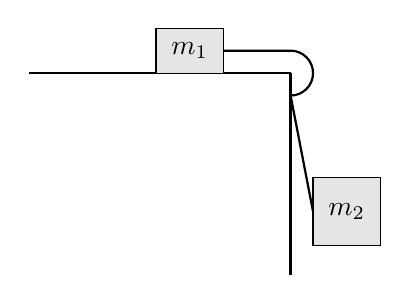
\begin{tikzpicture}[scale=0.95]
  \draw[thick] (-0.5,1.5) -- (3,1.5);
  \draw[thick] (3,1.5) -- (3,-1.2);
  \draw[fill=gray!20] (1.2,1.5) rectangle (2.1,2.1);
  \node at (1.65,1.8) {$m_1$};
  \draw[fill=gray!20] (3.3,-0.8) rectangle (4.2,0.1);
  \node at (3.75,-0.35) {$m_2$};
  \draw[thick] (2.1,1.8) -- (3,1.8) arc[start angle=90,end angle=-90,radius=0.3] -- (3.3,-0.35);
\end{tikzpicture}
\end{center}

\begin{solution}
设 $m_2$ 向下、$m_1$ 向右为正方向，二者加速度大小同为 $a$。

对 $m_1$：水平方向只有张力 $T$，故
\[
T=m_1 a.
\]
对 $m_2$：竖直方向有重力与张力，故
\[
m_2 g-T=m_2 a.
\]
联立得
\[
m_2 g=(m_1+m_2)a,
\qquad
a=\frac{m_2 g}{m_1+m_2}.
\]
张力为
\[
T=m_1 a=\frac{m_1m_2}{m_1+m_2}g.
\]
这类连接体问题的关键是：各物体分别列牛顿第二定律，再利用绳长不变得到加速度约束。
\end{solution}
\end{classic}

\begin{classic}
一质量为 $m$ 的小物块放在倾角为 $\theta$ 的光滑斜面上，并与沿斜面方向固定的一根轻弹簧相连，弹簧劲度系数为 $k$。开始时弹簧处于原长，放手后物块沿斜面下滑。

(1) 求平衡位置相对原长位置的位移；

(2) 以平衡位置为原点，写出运动微分方程；

(3) 求振动周期。

\begin{solution}
沿斜面向下取正。若弹簧伸长量为 $x$，则受力方程为
\[
m\ddot x=mg\sin\theta-kx.
\]
平衡位置满足 $\ddot x=0$，故
\[
kx_0=mg\sin\theta,
\qquad
x_0=\frac{mg\sin\theta}{k}.
\]
令
\[
\xi=x-x_0,
\]
则 $\ddot\xi=\ddot x$，代回上式得
\[
m\ddot\xi=mg\sin\theta-k(\xi+x_0)=mg\sin\theta-k\xi-kx_0=-k\xi.
\]
故运动方程化为
\[
\ddot\xi+\frac{k}{m}\xi=0.
\]
这是简谐振动方程，角频率为
\[
\omega=\sqrt{\frac{k}{m}},
\]
周期为
\[
T=2\pi\sqrt{\frac{m}{k}}.
\]
可见重力只改变平衡位置，不改变周期。这是“平移坐标消去恒力项”的典型思想。
\end{solution}
\end{classic}

\begin{classic}
电梯内一质量为 $m$ 的人站在体重计上。设电梯竖直向上为正方向，其位移满足
\[
z(t)=A\qty(1-\mathrm e^{-t/\tau}).
\]
试用微分方程方法求体重计示数 $N(t)$，并讨论初末状态。

\begin{solution}
由位移函数直接求加速度：
\[
\dot z=\frac{A}{\tau}\mathrm e^{-t/\tau},
\qquad
\ddot z=-\frac{A}{\tau^2}\mathrm e^{-t/\tau}.
\]
人受到重力 $mg$（向下）和支持力 $N$（向上），故牛顿第二定律为
\[
N-mg=m\ddot z.
\]
于是
\[
N(t)=m\qty(g-\frac{A}{\tau^2}\mathrm e^{-t/\tau}).
\]

当 $t=0$ 时，
\[
N(0)=m\qty(g-\frac{A}{\tau^2}).
\]
若 $A/\tau^2>0$，说明电梯初始加速度向下，因此体重计示数偏小。

当 $t\to\infty$ 时，
\[
N(\infty)=mg.
\]
因为此时电梯加速度趋于零，最终恢复匀速或静止状态，示数回到真实重力值。这个题目说明：所谓“超重”“失重”本质上是支持力偏离 $mg$，而不是重力真的改变。
\end{solution}
\end{classic}

\section*{竞赛题}

\begin{competition}
质量为 $m$ 的质点在光滑水平面上运动，受到外力
\[
F(t)=F_0\cos(\omega t)
\]
作用，初始条件为 $x(0)=0,\ v(0)=0$。

(1) 求速度与位移；

(2) 讨论当 $\omega\to 0$ 时的极限；

(3) 说明该模型与受迫振动的联系。

\begin{solution}
由牛顿第二定律
\[
m\dv{v}{t}=F_0\cos(\omega t)
\]
积分得
\[
v(t)=\frac{F_0}{m\omega}\sin(\omega t).
\]
再积分可得位移
\[
x(t)=\int_0^t \frac{F_0}{m\omega}\sin(\omega t')\,\dd t'
=\frac{F_0}{m\omega^2}\qty(1-\cos\omega t).
\]

当 $\omega\to 0$ 时，用 $\cos\omega t\approx 1-\omega^2 t^2/2$，得
\[
x(t)\approx \frac{F_0}{m\omega^2}\cdot \frac{\omega^2 t^2}{2}=\frac{F_0}{2m}t^2,
\]
这正是恒力作用下的匀加速直线运动结果。

若系统本身还带有回复力 $-kx$，则方程会变成
\[
m\ddot x+kx=F_0\cos\omega t,
\]
即标准受迫振动方程。故本题可以看成“无弹簧极限”的受迫问题。
\end{solution}
\end{competition}

\begin{competition}
一质量为 $m$ 的滑块从光滑水平面上以速度 $v_0$ 向右运动，撞上一根固定在墙上的轻弹簧，弹簧劲度系数为 $k$。设接触时弹簧原长，忽略一切耗散。

(1) 求压缩过程中滑块的运动方程与最大压缩量；

(2) 求从接触到再次离开弹簧所经历的时间；

(3) 说明“全过程”中速度、加速度的变化特点。

\begin{solution}
设弹簧压缩量为 $x$，接触瞬间 $t=0$，有
\[
x(0)=0,
\qquad
\dot x(0)=v_0.
\]
受力只有弹簧力 $-kx$，故
\[
m\ddot x+kx=0.
\]
角频率为 $\omega_0=\sqrt{k/m}$。满足初始条件的解为
\[
x(t)=\frac{v_0}{\omega_0}\sin(\omega_0 t),
\qquad
v(t)=\dot x=v_0\cos(\omega_0 t).
\]
当 $v=0$ 时压缩最大，因此
\[
\omega_0 t=\frac{\pi}{2},
\qquad
x_{\max}=\frac{v_0}{\omega_0}=v_0\sqrt{\frac{m}{k}}.
\]
这也可由机械能守恒得到：
\[
\frac12 mv_0^2=\frac12 kx_{\max}^2.
\]

再次离开弹簧对应 $x=0$ 的下一个时刻，即
\[
\omega_0 t=\pi,
\qquad
t_\text{离}=\frac{\pi}{\omega_0}=\pi\sqrt{\frac{m}{k}}.
\]

全过程中，速度从 $v_0$ 逐渐减小到 $0$，然后反向增大到 $-v_0$；加速度
\[
a=-\omega_0^2 x
\]
则从 $0$ 开始，逐渐变为向左的最大值，再回到 $0$。因此“最大形变对应最大加速度、零速度”，这是弹簧碰撞题的核心图像。
\end{solution}
\end{competition}

\begin{competition}
一根张紧的轻绳沿 $x$ 轴放置，线密度为 $\mu$，张力为 $T$。设横向微小位移为 $y(x,t)$。

(1) 用牛顿第二定律推导横波方程；

(2) 写出波速；

(3) 验证函数 $y=A\cos(kx-\omega t)$ 是其解，并给出色散关系。

\begin{solution}
取绳上一小段 $[x,x+\dd x]$，其质量为 $\mu\dd x$。在小振幅近似下，两端张力大小都近似为 $T$，竖直分量差为
\[
T\sin\theta\big|_{x+\dd x}-T\sin\theta\big|_x
\approx T\qty(\pdv{y}{x}\Big|_{x+\dd x}-\pdv{y}{x}\Big|_x)
= T\pdv[2]{y}{x}\dd x.
\]
对该微段使用牛顿第二定律：
\[
\mu\dd x\pdv[2]{y}{t}=T\pdv[2]{y}{x}\dd x.
\]
约去 $\dd x$，得到波动方程
\[
\pdv[2]{y}{t}=\frac{T}{\mu}\pdv[2]{y}{x}.
\]
故波速为
\[
v=\sqrt{\frac{T}{\mu}}.
\]

代入试探解
\[
y=A\cos(kx-\omega t)
\]
有
\[
\pdv[2]{y}{t}=-\omega^2 y,
\qquad
\pdv[2]{y}{x}=-k^2 y.
\]
因此必须满足
\[
\omega^2=\frac{T}{\mu}k^2.
\]
即
\[
\omega=vk,
\qquad
v=\sqrt{\frac{T}{\mu}}.
\]
这就是理想轻绳横波的色散关系。由于 $\omega$ 与 $k$ 成正比，它是无色散介质。
\end{solution}
\end{competition}

\section*{大学物理题}

\begin{university}
阻尼振子满足
\[
m\ddot x+b\dot x+kx=0,
\qquad b^2<4mk.
\]
试在相空间 $(x,v)$ 中分析其轨迹，并说明为何轨迹是向原点收缩的螺旋线。

\begin{solution}
欠阻尼条件下，令
\[
\gamma=\frac{b}{2m},
\qquad
\omega_d=\sqrt{\frac{k}{m}-\gamma^2},
\]
则通解可写为
\[
x(t)=A\mathrm e^{-\gamma t}\cos(\omega_d t-\phi).
\]
速度为
\[
v(t)=\dot x=-A\mathrm e^{-\gamma t}\qty[\gamma\cos(\omega_d t-\phi)+\omega_d\sin(\omega_d t-\phi)].
\]
如果没有阻尼，即 $b=0$，则机械能守恒，相轨迹为封闭椭圆。现在由于额外因子 $\mathrm e^{-\gamma t}$ 同时乘在 $x$ 与 $v$ 上，轨迹半径随时间指数衰减。

更深一层看，系统能量
\[
E=\frac12 mv^2+\frac12 kx^2
\]
满足
\[
\dv{E}{t}=mv\dot v+kx\dot x=v(m\dot v+kx)=-bv^2\le 0.
\]
故相轨迹不能向外发散，只能不断向能量更低的区域收缩。于是原来无阻尼的闭合轨线变成绕原点旋转并逐步靠近原点的螺旋线，最终停在稳定平衡点 $(0,0)$。
\end{solution}
\end{university}

\begin{university}
在一辆以恒加速度 $a_0$ 向右运动的车厢中，从某点以初速度 $v_0$ 竖直向上抛出一小球。相对车厢观察，求小球轨迹，并说明其形状。

\begin{solution}
在车厢参考系中，这是一个以加速度 $a_0$ 向右的非惯性系，因此小球除受重力外，还受到大小为 $ma_0$、方向向左的惯性力。故相对车厢的分运动满足
\[
\ddot x=-a_0,
\qquad
\ddot y=-g.
\]
初始条件为
\[
x(0)=0,\quad \dot x(0)=0,
\qquad
y(0)=0,\quad \dot y(0)=v_0.
\]
故
\[
x(t)=-\frac12 a_0 t^2,
\qquad
y(t)=v_0 t-\frac12 gt^2.
\]
由第一式解出
\[
t^2=-\frac{2x}{a_0}.
\]
再由第二式与参数形式联立，最直接的几何描述仍是参数方程。若消去 $t$ 的符号，可写成
\[
y=v_0\sqrt{-\frac{2x}{a_0}}+\frac{g}{a_0}x,
\qquad (x\le 0).
\]

因此在车厢内看，小球将向后方偏移，轨迹不再关于竖直线对称，而是一条向左弯曲的抛物型曲线。本质原因是非惯性系中的惯性力使水平方向出现恒定“伪加速度”。
\end{solution}
\end{university}

\begin{university}
理想 Atwood 机中，两端悬挂质量分别为 $m_1,m_2$ 的重物，设 $m_2>m_1$。

(1) 求系统加速度与绳张力；

(2) 用质心观点解释结果；

(3) 讨论极限情形 $m_1\to m_2$ 与 $m_1\ll m_2$。

\begin{solution}
设 $m_2$ 向下、$m_1$ 向上，二者加速度大小均为 $a$。分别列式：
\[
T-m_1 g=m_1 a,
\qquad
m_2 g-T=m_2 a.
\]
相加得
\[
(m_2-m_1)g=(m_1+m_2)a,
\qquad
a=\frac{m_2-m_1}{m_1+m_2}g.
\]
张力为
\[
T=m_1(g+a)=m_2(g-a)=\frac{2m_1m_2}{m_1+m_2}g.
\]

从整体看，系统总质量为 $m_1+m_2$，外力中能驱动系统运动的净力只有两边重力差
\[
F_\text{net}=(m_2-m_1)g.
\]
于是整体加速度自然为 $F_\text{net}/M$，这就是上式。张力则是内部约束力，用任一单体方程都能求出。

若 $m_1\to m_2$，则
\[
a\to 0,
\qquad T\to mg,
\]
系统近乎平衡。若 $m_1\ll m_2$，则
\[
a\to g,
\qquad T\to 0\text{（相对 }m_2g\text{ 而言很小）}.
\]
表示重的一端几乎自由下落，轻的一端几乎被“带着飞起”。
\end{solution}
\end{university}

\section*{普通/微分方程题}

\begin{problem}
设质点受一维速度依赖力 $F(v)$ 作用，满足
\[
m\dv{v}{t}=F(v).
\]

(1) 说明何时可以用分离变量法求解；

(2) 给出一般积分公式；

(3) 以 $F(v)=F_0-bv$ 为例写出完整解法。

\begin{solution}
只要 $F(v)$ 仅依赖于 $v$ 而不显含 $x,t$，并且在所讨论区间内连续，就可以把方程写成
\[
\frac{m\,\dd v}{F(v)}=\dd t,
\]
从而用分离变量法求解。积分得到一般隐式公式
\[
\int_{v_0}^{v(t)} \frac{m\,\dd u}{F(u)}=t.
\]
若该积分可反解，就能得到显式速度函数 $v(t)$。

进一步，位移可由
\[
x(t)=x_0+\int_0^t v(t')\,\dd t'
\]
求出。若更方便，也可利用
\[
\dv{x}{v}=\frac{\dv*{x}{t}}{\dv*{v}{t}}=\frac{v}{F(v)/m}=\frac{mv}{F(v)}
\]
从而直接得到 $x(v)$：
\[
x-x_0=\int_{v_0}^{v}\frac{mu}{F(u)}\,\dd u.
\]

以 $F(v)=F_0-bv$ 为例，速度方程为
\[
m\dv{v}{t}=F_0-bv.
\]
分离变量得
\[
\int_{v_0}^{v}\frac{m\,\dd u}{F_0-bu}=t.
\]
计算积分：
\[
-\frac{m}{b}\ln\frac{F_0-bv}{F_0-bv_0}=t.
\]
故
\[
v(t)=\frac{F_0}{b}+\qty(v_0-\frac{F_0}{b})\mathrm e^{-bt/m}.
\]
这正对应“趋于终端速度 $F_0/b$”的一般规律。
\end{solution}
\end{problem}

\begin{problem}
设一维运动中合力仅与位置有关，即 $F=F(x)$。

(1) 从牛顿第二定律出发推导能量方法；

(2) 说明稳定平衡点与势能极小值的关系；

(3) 以 $F(x)=-kx+\beta x^3$ 为例写出势能函数。

\begin{solution}
牛顿第二定律为
\[
m\ddot x=F(x).
\]
两边乘以速度 $\dot x$：
\[
m\ddot x\dot x=F(x)\dot x.
\]
左边可识别为
\[
\frac{\dd}{\dd t}\qty(\frac12 m\dot x^2),
\]
右边则是
\[
F(x)\dv{x}{t}=\dv{}{t}\qty(\int F(x)\,\dd x).
\]
于是
\[
\frac{\dd}{\dd t}\qty(\frac12 m\dot x^2-\int F(x)\,\dd x)=0.
\]
定义势能函数
\[
U(x)=-\int F(x)\,\dd x,
\]
便得到机械能守恒
\[
\frac12 m\dot x^2+U(x)=E.
\]

平衡点满足 $F(x_0)=0$，即 $U'(x_0)=0$。若进一步有
\[
U''(x_0)>0,
\]
则 $x_0$ 为势能极小值，对应稳定平衡；若 $U''(x_0)<0$，则为极大值，对应不稳定平衡。

对
\[
F(x)=-kx+\beta x^3
\]
有
\[
U(x)=-\int(-kx+\beta x^3)\,\dd x=\frac12 kx^2-\frac14 \beta x^4+C.
\]
若取 $C=0$，则
\[
U(x)=\frac12 kx^2-\frac14 \beta x^4.
\]
这个势能在小位移时近似抛物线，但远处可能因四次项而发生形状改变，因此能量法特别适合分析其允许运动区域与转折点。
\end{solution}
\end{problem}
